\section{Results}
\label{sec:results}

% Held-out evaluation metrics (2025-2026, n=207).
% Source: analysis/outputs/tables/holdout_metrics.csv
% Spearman rho not defined for global median (constant predictions).
\begin{table}[t]
\centering
\caption{Held-out evaluation on 2025--2026 seasons ($n=207$). Spearman $\rho$ undefined for the global median baseline (constant predictions).}
\label{tab:holdout-metrics}
\small
\setlength{\tabcolsep}{4pt}
\begin{tabular}{lrrrr}
\toprule
Model & MAE & RMSE & $R^2$ & Spearman $\rho$ \\
\midrule
Global median       & 5.858 & 7.291 & $-0.004$ & --- \\
Class median        & 4.767 & 5.932 & 0.336  & 0.568 \\
Debut score         & 11.271 & 12.279 & $-1.847$ & 0.733 \\
\midrule
Ridge               & \textbf{2.676} & \textbf{3.499} & \textbf{0.769} & \textbf{0.892} \\
Gradient boosting   & 2.934 & 3.805 & 0.727 & 0.868 \\
\bottomrule
\end{tabular}
\end{table}


Table~\ref{tab:holdout-metrics} reports held-out evaluation metrics for all
models on the 2025--2026 seasons ($n = 207$). The global-median baseline
achieves an MAE of 5.858 and an $R^2$ near zero, consistent with constant
predictions. The class-median baseline substantially improves on it (MAE
4.767, Spearman $\rho = 0.568$), confirming that class membership carries
predictive information beyond a global constant. The debut-score identity
baseline preserves meaningful rank ordering (Spearman $\rho = 0.733$) but
severely underpredicts terminal scores, with a mean residual of $-11.224$
points; ensembles improve considerably between debut and championship, so the
raw debut score is a poor terminal-score forecast.

Ridge regression achieves a held-out MAE of 2.676 (RMSE 3.499, $R^2 = 0.769$,
Spearman $\rho = 0.892$). Ridge was selected as the headline model by
development cross-validation MAE (2.769) rather than by post-hoc holdout
comparison. A cluster bootstrap 95\% confidence interval for the
difference GBM MAE $-$ Ridge MAE is $[0.056, 0.454]$ (2,000 resamples, clustered by ensemble identity), confirming that Ridge
outperforms gradient boosting on this evaluation. Gradient boosting's weaker
held-out performance is consistent with the structure of the task: the ablation
and Ridge coefficient analysis both indicate that debut subtotal and class
membership account for most of the predictive signal, leaving little residual
structure for an ensemble method to exploit. At 574 development observations,
the added complexity of gradient boosting does not recover additional signal
over Ridge. An empirical prediction
interval formed by adding and subtracting the development residual 90th
percentile (5.795 points) covers 87.9\% of held-out outcomes.
Figure~\ref{fig:predicted-vs-observed} shows predicted versus observed
subtotals for the Ridge model.

% Ridge regression: predicted vs. observed terminal championship subtotal.
% Data: ../analysis/outputs/tables/holdout_predictions.csv (207 held-out rows, 2025-2026).
\begin{figure}[t]
\centering
\pgfplotstableread[col sep=comma]{../analysis/outputs/tables/holdout_predictions.csv}\holdout
\begin{tikzpicture}
\begin{axis}[
  width=\columnwidth,
  height=5.8cm,
  xlabel={Predicted subtotal},
  ylabel={Observed subtotal},
  xlabel style={font=\small},
  ylabel style={font=\small},
  tick label style={font=\small},
  xmin=62, xmax=100,
  ymin=62, ymax=100,
  xtick={65,70,75,80,85,90,95,100},
  ytick={65,70,75,80,85,90,95,100},
  grid=major,
  grid style={dotted, gray!40},
]
\addplot[
  only marks,
  mark=o,
  mark size=1.4pt,
  mark options={fill=black!60, draw=black!60},
  opacity=0.65,
] table[x=ridge_prediction, y=terminal_subtotal_score]{\holdout};
\addplot[
  domain=62:100,
  thick,
  dashed,
  black!50,
] {x};
\end{axis}
\end{tikzpicture}
\caption{Ridge regression: predicted vs.\ observed terminal championship subtotal on the 2025--2026 held-out set ($n=207$). The dashed line marks perfect prediction. MAE $=2.676$, $R^2=0.769$.}
\Description{Scatter plot of predicted against observed championship subtotals. Most points lie near the diagonal perfect-prediction line, with wider errors among lower scores.}
\label{fig:predicted-vs-observed}
\end{figure}


% Ablation study: expanding-season development CV MAE for each feature block.
% Source: analysis/outputs/tables/ablation.csv
% Validation folds: train on 2017, predict 2018; add seasons through 2024.
\begin{table}[t]
\centering
\caption{Ablation results: Ridge development CV MAE as feature blocks are added sequentially. Each block adds only the indicated features to the previous set.}
\label{tab:ablation}
\small
\setlength{\tabcolsep}{4pt}
\begin{tabular}{lrr}
\toprule
Feature set & Features & Dev CV MAE \\
\midrule
A: debut subtotal only          &  1 & 3.551 \\
B: + timing and class           &  6 & 3.060 \\
C: + competition context        & 10 & 2.876 \\
D: + score profile              & 26 & 2.921 \\
E: + prior history              & 31 & \textbf{2.798} \\
F: + class-change direction      & 33 & 2.798 \\
\bottomrule
\end{tabular}
\end{table}


Table~\ref{tab:ablation} reports development cross-validation MAE for each
ablation step. Adding debut timing and class (B) produces the largest
single-step improvement. Competition context (C) adds further gain; the
score-profile block (D) does not improve over C at this sample size; prior
history (E) recovers the gap; and explicit class-change direction (F)
adds no further improvement. Figure~\ref{fig:ridge-coefficients} shows the 15
largest Ridge coefficients by absolute magnitude. PIA (the lowest-tier
independent class) is the regression reference category; this choice scales
coefficient magnitudes relative to that baseline but does not affect model
predictions or any reported metric. Debut subtotal and class membership are
the dominant predictors; prior championship subtotal adds incremental signal.

% Ridge held-out MAE and median residual by class.
% Source: analysis/outputs/tables/holdout_by_class.csv
% ridge_bias = mean residual (predicted - observed); ridge_median_residual = median residual.
% Class names spelled out: Independent A/Open/World, Scholastic A/Junior/Open/World.
\begin{table}[t]
\centering
\caption{Class-level Ridge error; median residual separates bias from dispersion.}
\label{tab:holdout-by-class}
\small
\setlength{\tabcolsep}{4pt}
\begin{tabular}{lrrrr}
\toprule
Class & $n$ & MAE & Mean bias & Median resid. \\
\midrule
PIA (Ind.\ A)       &   6 & 1.158 & $+$0.408 & $+$0.542 \\
PIO (Ind.\ Open)    &   2 & 1.579 & $+$0.384 & $+$0.384 \\
PIW (Ind.\ World)   &  14 & 1.402 & $+$0.563 & $+$0.176 \\
PSA (Sch.\ A)       & 112 & 3.254 & $+$0.512 & $+$0.087 \\
PSJ (Sch.\ Junior)  &  17 & 2.425 & $-$0.990 & $-$1.398 \\
PSO (Sch.\ Open)    &  41 & 2.451 & $+$0.348 & $+$0.387 \\
PSW (Sch.\ World)   &  15 & 1.196 & $-$0.356 & $-$0.580 \\
\bottomrule
\end{tabular}
\end{table}


Table~\ref{tab:holdout-by-class} disaggregates held-out MAE and residuals by
class. PSA (Scholastic A) has the highest class-level MAE (3.254 across 112
held-out observations, 54.1\% of the holdout). Its near-zero median residual
($+0.087$), widest terminal-score (SD 6.764) and residual (SD 4.101)
distributions, and large errors in both directions indicate heterogeneous
development rather than systematic overprediction. PSA supplies eight of the
ten largest positive residuals, partly reflecting its sample size.

% Ridge regression coefficients — top 15 by absolute value.
% Values hardcoded from analysis/outputs/tables/ridge_coefficients.csv (frozen outputs).
% Sorted bottom-to-top (index 0 = most negative, index 14 = most positive).
% Uses numeric y-axis with yticklabels to avoid pgfplots symbolic-coord parser issues
% with parentheses in label names.
\begin{figure}[t]
\centering
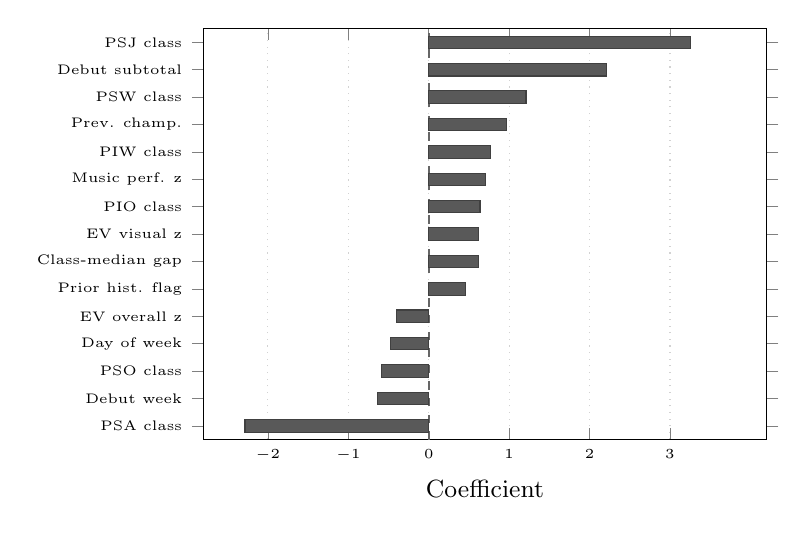
\begin{tikzpicture}
\begin{axis}[
  xbar,
  width=0.72\columnwidth,
  height=6.8cm,
  bar width=4.5pt,
  xlabel={Coefficient},
  xlabel style={font=\small},
  tick label style={font=\tiny},
  xmin=-2.8, xmax=4.2,
  xtick={-2,-1,0,1,2,3},
  ymin=-0.5, ymax=14.5,
  ytick={0,1,2,3,4,5,6,7,8,9,10,11,12,13,14},
  yticklabels={
    PSA class,
    Debut week,
    PSO class,
    Day of week,
    EV overall z,
    Prior hist. flag,
    Class-median gap,
    EV visual z,
    PIO class,
    Music perf. z,
    PIW class,
    Prev. champ.,
    PSW class,
    Debut subtotal,
    PSJ class,
  },
  xmajorgrids=true,
  grid style={dotted, gray!35},
  extra x ticks={0},
  extra x tick labels={},
  extra x tick style={
    grid=major,
    grid style={black!60, dashed, line width=0.7pt},
    tick style={draw=none},
  },
]
\addplot[
  fill=black!65,
  draw=black!75,
] coordinates {
  (-2.2845,0)
  (-0.6380,1)
  (-0.5830,2)
  (-0.4727,3)
  (-0.4000,4)
  (0.4579,5)
  (0.6232,6)
  (0.6234,7)
  (0.6378,8)
  (0.7016,9)
  (0.7704,10)
  (0.9724,11)
  (1.2092,12)
  (2.2151,13)
  (3.2527,14)
};
\end{axis}
\end{tikzpicture}
\caption{Top 15 Ridge regression coefficients by absolute magnitude. Class coefficients are relative to PIA, the omitted reference category; reference class choice affects coefficient scale but not model predictions. Positive values indicate higher predicted championship subtotal; negative indicate lower. Debut subtotal and class membership dominate; prior championship subtotal adds incremental signal.}
\Description{Horizontal bar chart of the 15 largest standardized Ridge coefficients. Debut subtotal and several class indicators have the largest magnitudes.}
\label{fig:ridge-coefficients}
\end{figure}

